\documentclass[11pt, a4paper,twocolumn]{jarticle}
\usepackage[dvipdfmx]{graphicx}
\usepackage{listings,jlisting}

\begin{document}
%=============================================================
\section{ステッピングモーターの動作確認}
\subsection{目的}
今回の実験では走査状態での信号読み取りを行うためにプログラムを用いてパソコンでステッピングモーターを制御する方法を理解する.

\subsection{手順}
まず前回の実験でレーザー入力する電圧を制御しするプログラムを流用して矩形波を作り出すプログラムを作成した.
次にプログラムを用いて矩形波信号の周波数を1kHz,500Hzにしてデューティー比を1:1に設定してモーターの回転角を求めた.
次に周波数が250Hzでデューティー比が1:3の矩形波とデューティー比が3:1の矩形波について同様に回転角を求めた.
またこれらの実験では$2\times{10^4}$個のデータ配列を用いて,サンプリング周波数を2kHzに設定した.

\subsection{結果}
測定の結果各矩形波についての回転角は表\ref{fig:hogehoge}のようになった.

\begin{table}[ht]
\centering
\caption{光信号の取り込み}
\label{my-label}
\begin{tabular}{c c c}
\hline
周波数[Hz] & 回転時間[s] & 回転角[deg] \\ \hline
1000 & 10 & 102 \\
500 & 20 & 102 \\
250 & 10 & 51 \\
250 & 10 & 51 \\
\end{tabular}
\label{fig:hogehoge}
\end{table}

\newpage


\subsection{考察}
実験の結果よりステッピングモーター回転角は入力信号のデューティー比には関係がなく,読み込んだ矩形波の数(周波数と回転時間の積)によってのみ決まると予想できる.
また回転速度を上げたければサンプリング周波数を大きくすればよく,回転時間を長くしたければデータ配列を大きく取れば良いと予想される.
ここで矩形波1周期分の回転角は実験結果より
\begin{equation}
    \frac{104[deg]}{1000 \times10[s]} = 1.02 \times{10^{-2}}[deg]
\end{equation}
と計算できる.

また図\ref{fig:6}に示すようにレーザーが凸レンズの中心付近を通った際には入力物体上での読み取りピッチ$\Delta x$は以下のように表せる.
\begin{eqnarray}
    \Delta{x} &=& ftan{\theta} \\
    &\sim& f\theta
\end{eqnarray}
以上の式より今回測定した1周期あたりの回転角度を考慮して今回の実験光学系での読み取りピッチを計算すると$1.78\times{10^{-2}}$[mm]となる.
またこの近似式はレンズの中心を離れるほど誤差は大きくなりより$\Delta{x}$は大きくなる.

\begin{figure}[ht]
 \begin{center}
  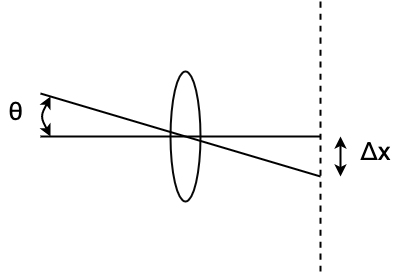
\includegraphics[width=0.8\linewidth]{fig6.png}
 \end{center}
 \caption{光学系}
 \label{fig:6}
\end{figure}

%=============================================================
\newpage
\end{document}
